\documentclass[addpoints]{exam}
\usepackage[utf8]{inputenc}
\usepackage[portuguese]{babel}
\usepackage[LGRgreek]{mathastext}
\usepackage{graphicx,graphics}
\usepackage{hyperref}

\footer{}{\thepage}{}
 
\pointpoints{ponto}{pontos}
\bonuspointpoints{ponto extra}{pontos extra}
 
\totalformat{Pregunta \thequestion: \totalpoints pontos}
 
\chqword{Pregunta}
\chpgword{Página}
\chpword{Pontos}
\chbpword{Pontos extra}
\chsword{Pontos obtidos}
\chtword{Total}

\hqword{Questão}
\hpgword{Página}
\hpword{Pontos}
\hsword{Pontos obtidos}
\htword{Total}

 
\begin{document}
 
\begin{center}
Eletrônica Básica II – EE640 U - Lista SPICE 1
\end{center}
 
\vspace{5mm}
 
\noindent\makebox[0.72\textwidth]{Nome: \enspace\hrulefill}
\hfill
\makebox[0.2\textwidth]{RA: \enspace\hrulefill}

\vspace{2mm}

\noindent\makebox[0.72\textwidth]{Nome: \enspace\hrulefill}
\hfill
\makebox[0.2\textwidth]{RA: \enspace\hrulefill}

\vspace{2mm}

\noindent\makebox[0.72\textwidth]{Nome: \enspace\hrulefill}
\hfill
\makebox[0.2\textwidth]{RA: \enspace\hrulefill}

\vspace{2mm}

\noindent\makebox[0.72\textwidth]{Nome: \enspace\hrulefill}
\hfill
\makebox[0.2\textwidth]{RA: \enspace\hrulefill}

\begin{center}
A lista deve ser entregue até dia \textbf{01-01-1968}

\vspace{5mm}

Use o seu RA como \textit{\textbf{abcdef}}, exemplo: para 123456, ab=12, ef=56 e assim port diante.

Utilize 0 como 10, 00 como 100. RA = 002220, ab=100, f=10.

\vspace{2mm}

\textbf{Para resolução deverá ser usado o maior RA do grupo.}

\end{center}

\begin{center}
\gradetable[h][questions]
\end{center}

\hspace{2mm}

\begin{questions}

\question Usando o \textit{software} de circuitos, faça a simulação do amplificador observando os critérios abaixo O modelo do transistor deve obrigatoriamente ser alterado. Use os seguintes parâmetros:

.model MbreakP-M PMOS vto=-0.5 l=1u kp=10u lambda=0.01 cbd=1p cgdo=1f cgso=1f

.model MbreakP-M PMOS vto=0.5 l=1u kp=10u lambda=0.01 cbd=1p cgdo=1f cgso=1f

\vspace{2mm}

\begin{parts}
\part[1] No circuito abaixo, identifique as seguintes partes: Fonte de Corrente, Espelho de Corrente, Carga Ativa e Estágio de entrada.
\part[1] Calcule o valor de $R_1$ para que a corrente de referência ($I_{REF}$) seja 10 $\mu A$ + ``ef''$\times10^{-7}$.
\part[1] Dimensione o primeiro estágio para um ganho de tensão total de 100 + ``cd''.
\part[2] Obtenha as curvas de módulo e fase da resposta em frequência de 1 Hz a 1 GHz.
\part[2] Obtenha os valores quiescentes (cc) de corrente e tensão no circuito.
\end{parts}

\begin{center}
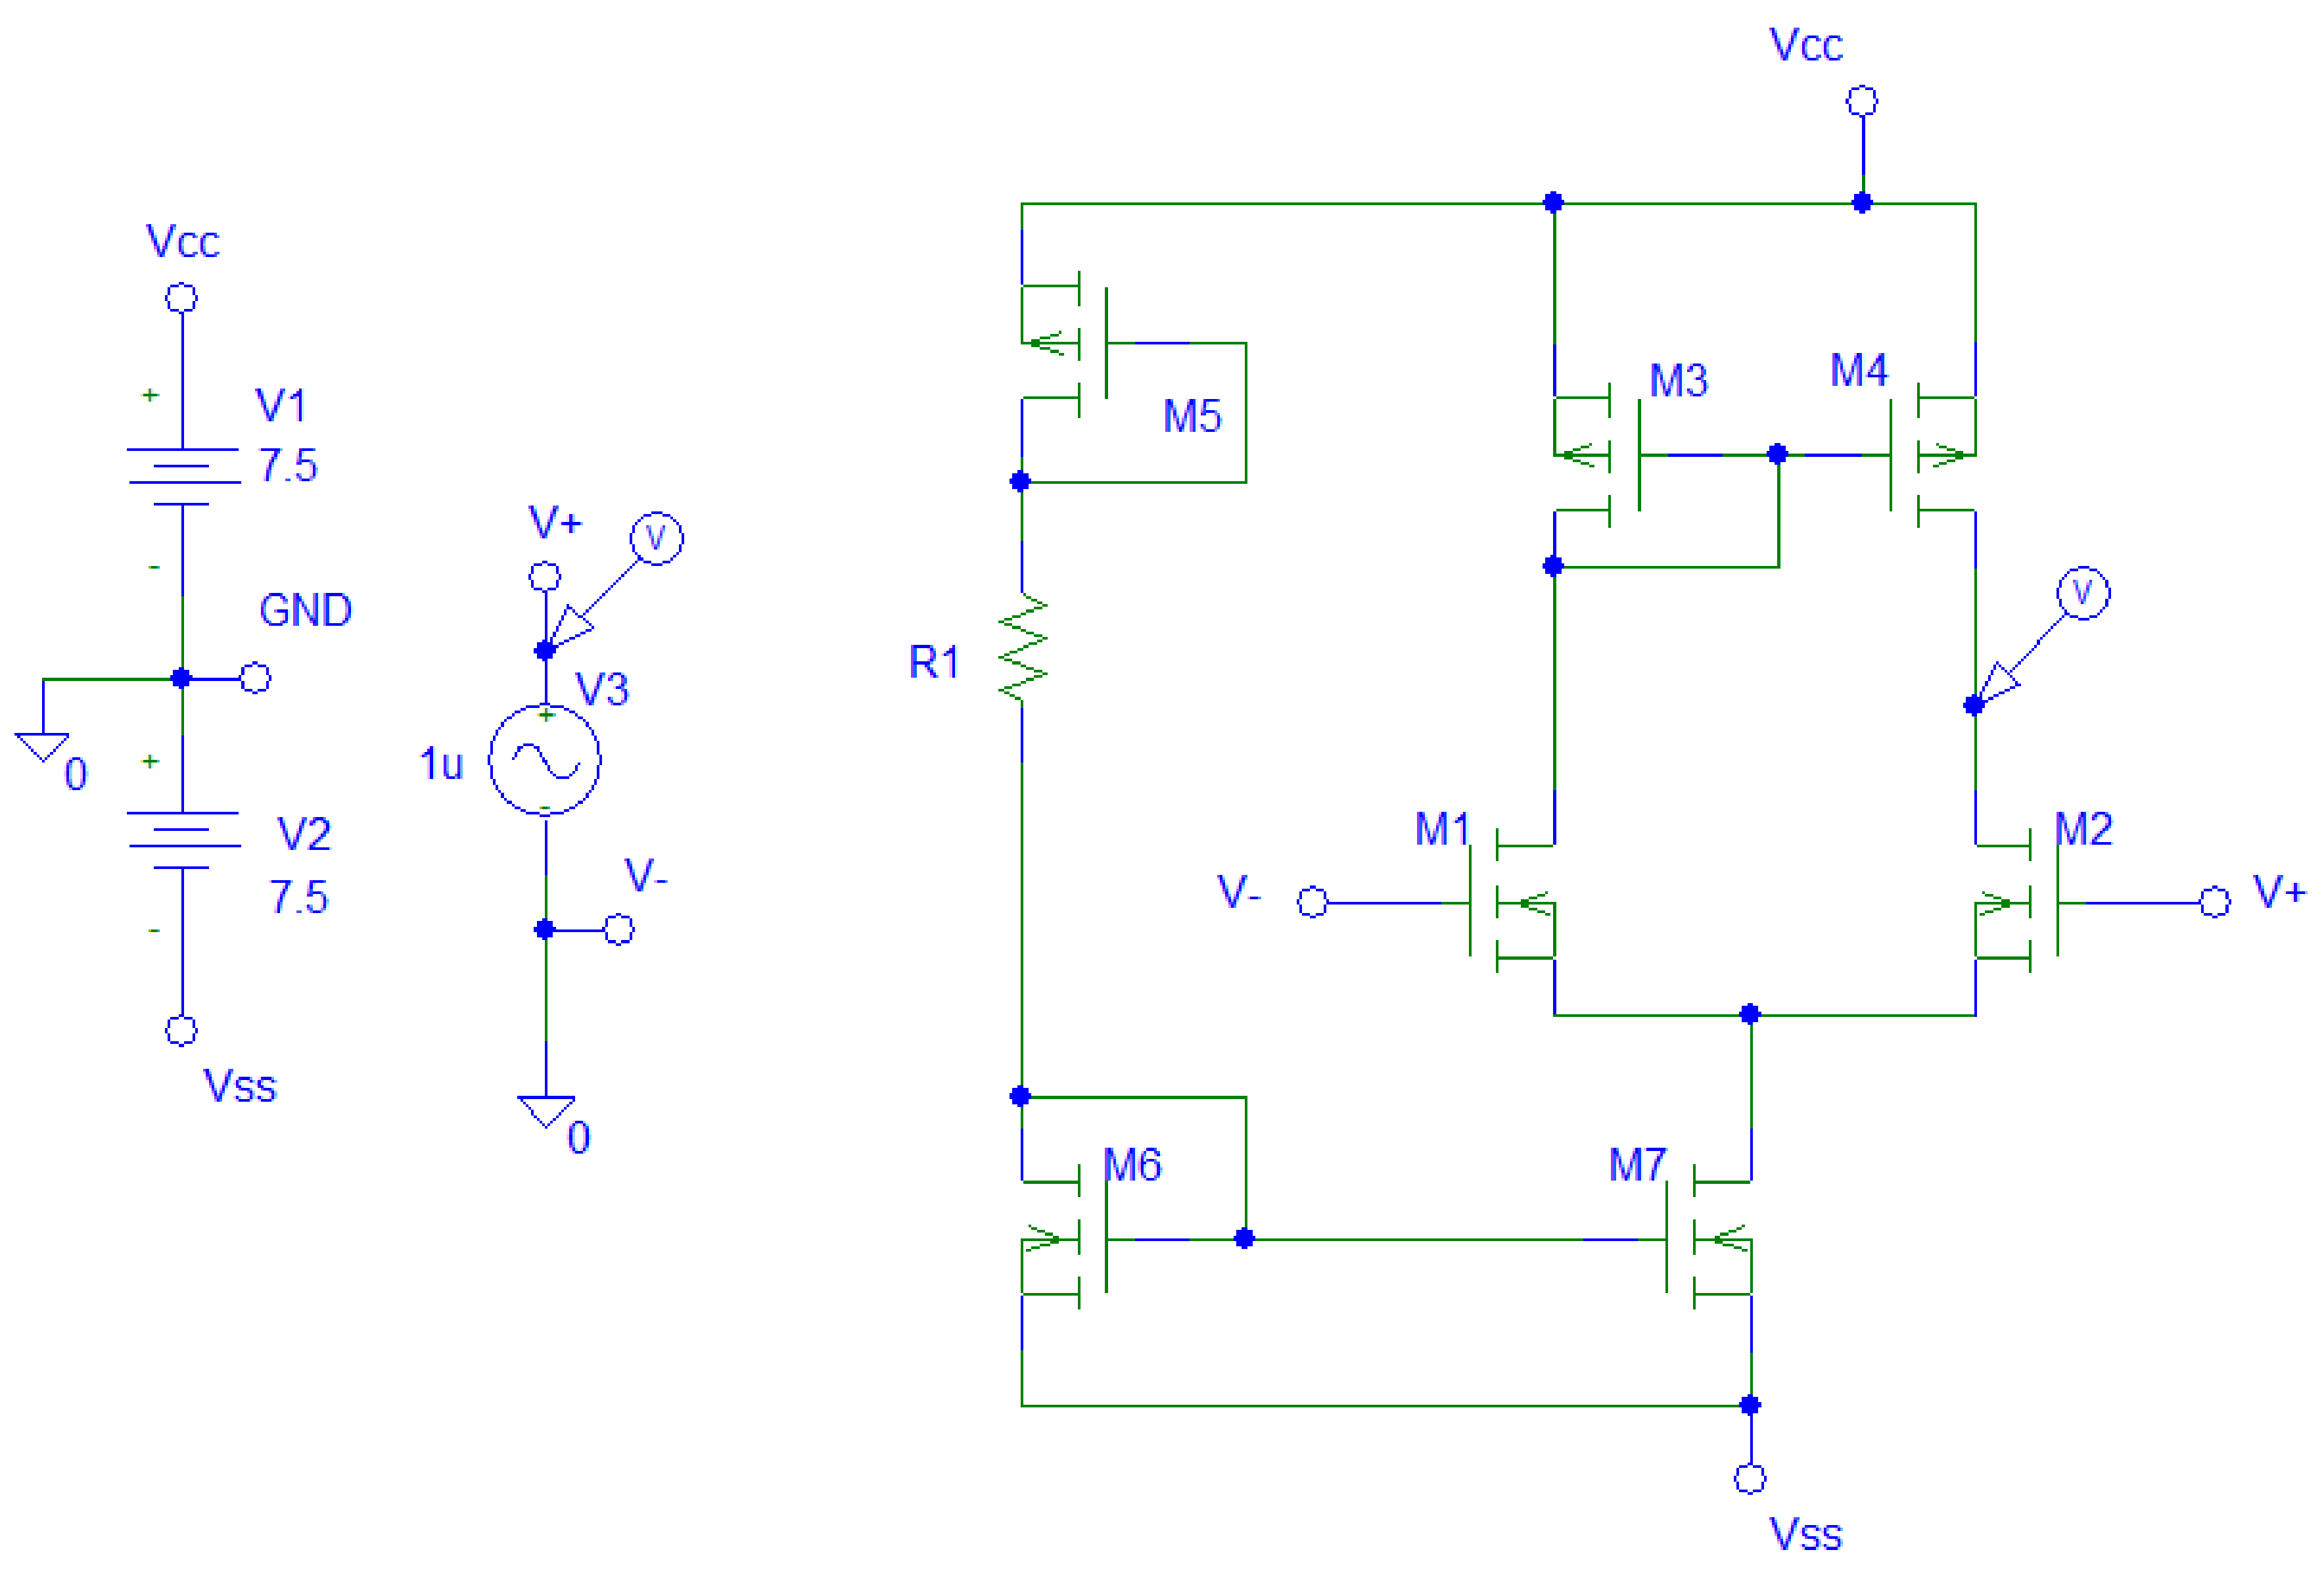
\includegraphics[width=0.7\textwidth]{imagens/1.png} 
\end{center}

\vspace{5mm}

\textbf{REFERÊNCIAS}

\vspace{5mm}

MANERA, Leandro T. \textbf{Vídeos sobre SPICE}. \url{http://www.dsif.fee.unicamp.br/~manera/EE640/download.html}. Acesso em 08-01-2019.

UNIVERSITY OF PENNSYLVANIA. \textbf{Spice model parameters of mosfets}. \url{https://www.seas.upenn.edu/~jan/spice/spice.MOSparamlist.html}. Acesso em 08-01-2019.

\end{questions}

\end{document}
